\chapter{Our Approach}
\label{proposedsolution}
In this chapter we present our solution to the puzzle solving problem. The proposed solution takes into account IDA*, MCTS and some enhancements of standard versions of these algorithms. We describe the enhancements implemented and added to the basic algorithms and to Sokoban. First, we describe the implemented IDA* optimizations; next we describe optimizations for the MCTS algorithm. The enhancements are either domain independent, which can be applied to each algorithm and to both the considered domains, or domain dependent, specific for the different domains.

\section{IDA* optimizations}
The performance of IDA* is strongly tied to the quality of the heuristic evaluation, however there are techniques that can improve the results under certain conditions by reducing the size of the search tree or the order in which nodes are explored.

\subsection{Transposition Tables}
Transposition tables are a data structure that keeps track of the visited states in order to reduce the branching factor of the game tree. The assumption at the base of the use of transposition tables is that the same state can be reached through different paths. When this assumption holds, transposition tables can be used to avoid cycles during the search by expanding only nodes that represent a state that has not yet been visited. In addition to cycles avoidance, we can use transposition tables to prune sub-trees according to the outcome of previous searches.

\medskip\noindent
A transposition table requires: an entry, a record that represent the state and data relevant to the search; an hash table, the actual table that holds an entry in each cell.
\begin{figure}[ht]
\centering
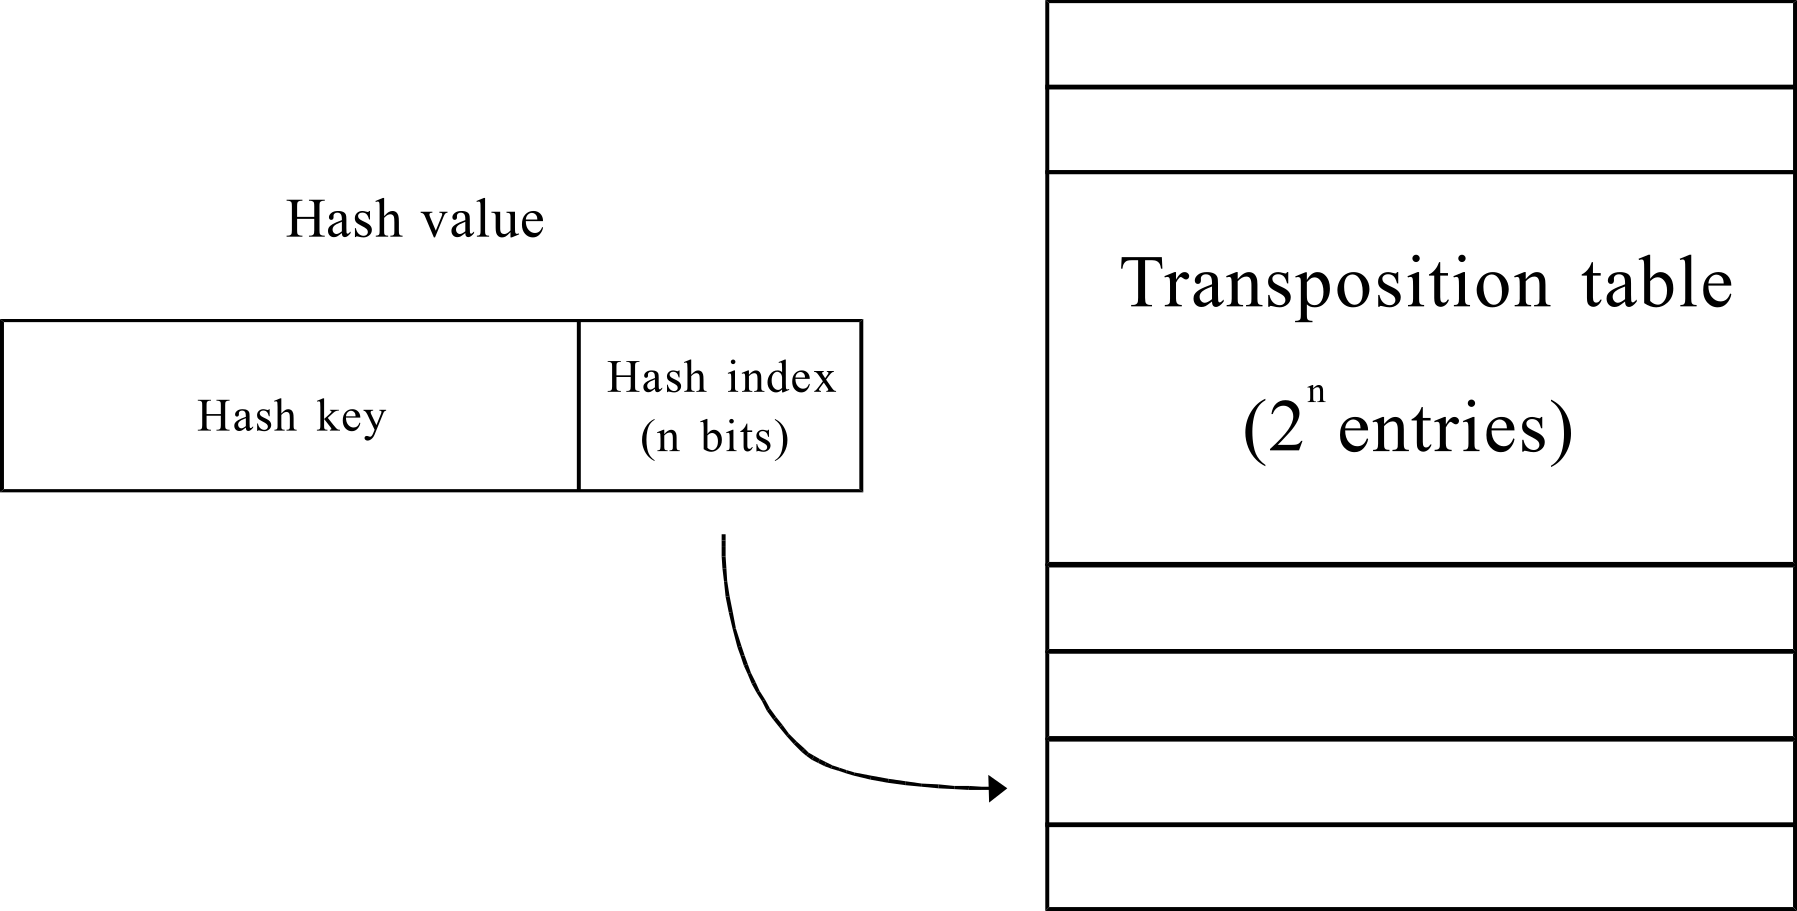
\includegraphics[width=0.6\linewidth]{pictures/TranspositionTable.png}
\caption[Hash Table]{Hash Table \cite{transpositiontables}}
\label{fig:transpositiontable}
\end{figure}

\medskip\noindent
Figure \ref{fig:transpositiontable} shows the typical usage of transposition tables. The hash value is computed through an hash function specifically built for the domain we are considering. The perfect hash function should be built in such a way that two states that should be considered different for the search purpose have different hash values, while two state that should be considered equivalent have the same hash value. Once computed, the \textit{hash index}, a portion of the hash value of a state, is used as an index to access the table, while either the remaining portion of the hash called \textit{hash key}, or the full hash value is stored inside the table to handle collisions that might happen between different states that map onto the same index.
Therefore, the table entry should contain the either the hash key or the hash value, along with all data that is relevant to the search. In the case of IDA*, this data include
\begin{itemize}
    \item \textit{Score}: the heuristic value obtained in previous visit through the state. When the state is first added to the transposition table, the score should be its heuristic value. Once the sub-tree that starts from the state has been completely explored up to the threshold, the score oh the state should be updated with the score obtained further along the search, since it's supposed to be more accurate. In the case of IDA*, it's computed as the minimum value among the successors of the current node.
    \item \textit{Depth}: the relative depth of the explored sub-tree. This represents how deep the tree has been explored, starting from the current state. In the context of IDA*, the depth can be computed as $threshold-g$, where $threshold$ is the threshold of the current iteration and $g$ is the cost of the path from the root state to the current state.
    \item \textit{Visited}: a flag that represent whether the entry is part of the current path or it has been added in a previous search. This allows us to discern between cycle avoidance and tree pruning.
\end{itemize}

\medskip\noindent
In an ideal setting, the transposition table size would be enough to hold every state visited during the search. In real applications, such as Samegame and Sokoban, with large branching factors, we limit the size of the table as shown in Figure \ref{fig:transpositiontable}. A replacement scheme represent the policy used to handle conflicts. The replacement scheme defines whether upon collision, the entry contained in the table should be kept or should be replaced with the new entry. Breuker \cite{transpositiontables} examined several different replacement schemes based on different concepts:
\begin{itemize}
    \item \textit{Deep}: The entry with the largest depth is kept in the table. The rationale behind this scheme is that the sub-tree associated to an entry with a great depth contains more nodes than the lower depth one, thus containing more accurate information and saving more work in case of pruning.
    \item \textit{New}: The newest entry is kept in the tree. This scheme is based on the observation that most transposition occur in local sub-trees, implying that keeping most recent nodes in the transposition table allows us to prune more often.
    \item \textit{Old}: The oldest entry is kept in the tree. No replacement occurs. The author included this scheme only for the sake of completeness.
    \item \textit{Big}: The entry with the largest amount of nodes in the sub-tree is kept in memory. This is similar to the Deep scheme and might perform better when the depth is not a good estimator of the size of the sub-tree, but requires to keep in the entry also the number of nodes, effectively reducing the number of entry that can be stored in the table.
    \item \textit{Two-Level}: The transposition table is organized in two levels and the replacement scheme is combined with one of the above. The the main replacement scheme is applied with the selected entry stored in the first level of the table, while the entry that would normally be discarded is stored on the second level. When retrieving the entry, the second table is used only if there's no match in the first table. This scheme allows us to store both more recent (to increase the number of hits) and more informative entries (to prune large sub-trees). Note however that keeping two tables imply that the number of entry stored for each table is halved.
\end{itemize}
Breuker \cite{transpositiontables} results showed that the two-level replacement scheme obtains the highest reduction in number of explored nodes, with its Big combination having a slight edge over the Deep one. We decided however to follow Junghanns et al. \cite{Junghanns99pushingthe} example and implemented a two-level transposition table based on depth, since it lends itself well for use with IDA*, as depth can be computed before actually exploring the sub-tree, as mentioned earlier.

\medskip\noindent
As we already mentioned, the effect of transposition tables on IDA* is two-fold: cycles avoidance and tree pruning.
In practice, the search explores a new node, it first checks the transposition table for an entry with the same state. If one is found and its depth is greater than the current estimated depth, the node is not explored further and its value is returned as the score of the entry. Otherwise, the a new entry is stored and the search continues among the successors (Algorithm \ref{alg:idastar}), with the exception that only child nodes that do not appear as visited are explored.

\subsection{Move ordering}
IDA* explores in a depth first manner, so if the algorithm explores promising nodes first, it will find a solution faster. Following this idea, move ordering sorts the available moves before expansion according to a certain criterion. This criterion can be domain dependent, as in \cite{Junghanns99pushingthe}, or domain independent, as in \cite{DBLP:journals/pami/ReinefeldM94}. We decided to implement move ordering with a domain independent ordering criterion by sorting the moves according to the heuristic evaluation of the resulting state.
\medskip\noindent
Since in IDA* all iterations except for the last one perform a complete search, the only contribution of move ordering is visible on the last iteration, but since that is the largest one by number of nodes, if the solution is found in an earlier sub-tree it may reduce execution time by a significant amount.

\section{MCTS configuration}\label{rewardtype}
To identify a specific MCTS configuration we need to define simulation policies and the rewards used. We defined four different reward types for Sokoban:

\begin{enumerate}
    \item \textit{R0}: 1 if the state represents a solved level, 0 otherwise.
    \item \textit{Boxes}: the reward is the same as the one used by \cite{DBLP:journals/corr/WeberRRBGRBVHLP17} and is computed as
    \begin{equation}
        r = 0.1\times steps + b_{ON} - b_{OFF} + solved 
    \end{equation}where $steps$ is the number of pushes executed, $b_{ON}$ is the number of times a box has been pushed on a goal, $b_{OFF}$ is the number of times a box has been pushed off a goal and $solved$ is 10 if the level is solved, 0 otherwise.
    \item \textit{InverseBM}: $1/\sqrt{BM}$, where $BM$ is the \textit{minimum cost perfect matching on a complete bipartite graph}, i.e. the minimum sum of the distances from each box to its designated goal. $BM$ is the heuristic evaluation used by \cite{Junghanns99pushingthe}. This reward has the advantage of having values in the range \{0,1\}.
    \item \textit{NegativeBM}: $-BM$. This reward has values in the range \{$-\infty$,0\}, but has the advantage of the linearity of the reward.
\end{enumerate}

\medskip\noindent
We tested different simulation policies:
\begin{itemize}
    \item \textit{random}: selects a random action among those available in the current state.
    \item \textit{$\epsilon$-greedy}: selects a random action with probability $\epsilon$ or the action that maximizes the reward of the resulting state with probability $1-\epsilon$.
    \item \textit{$\epsilon$-IDA*}: selects a random action with probability $\epsilon$ or -- with probability $(1-\epsilon)$ -- perform an IDA* search with a limited number of nodes and return the first action of the path that leads to the state with the lowest heuristic value. For this policy we tested different configurations in terms of number of IDA* nodes and MCTS iterations.
\end{itemize}
For the backpropagation policy, in addition to the usual sum of rewards and number of visits we stored the maximum score, the sum of the squared rewards and the sum of rewards and visits for the RAVE optimization (Section \ref{sec:rave}). The winning action is the one with the highest maximum score.

\section{MCTS optimizations}
Standard version of the core MCTS algorithm can be applied to various domains due to its main characteristic of not requiring domain-specific knowledge, but when it is needed to compare it - in a specific domain - with another artificial intelligence modified in order to have good performance in such domain, it can work not so well. In order to achieve better results in this kind of comparison, we need to modify the standard algorithm introducing some enhancements in order to improve performance.

\medskip\noindent
In the proposed solution all enhancements are domain independent, so can be applied to any domain without prior knowledge about it, this choice is done in order to have a unique optimized MCTS algorithm that can be used in each game considered in this work without the need of any change due to some specific knowledge.

\subsection{Object Pooling}
The Object Pool pattern is a software creational design pattern used to improve memory usage and performance. This pattern uses a set of initialized objects kept ready to use --- also called ``pool'' --- rather than allocating and destroying them on demand. In order to use this pool, it is possible to require an object from it and then perform operations on the returned object. When the object is not used anymore, it can be returned to the pool, in order to have the possibility to use it again later, rather than destroying it; this can be done manually or automatically.

\medskip\noindent
The MCTS algorithm can create a large number of objects that are particularly expensive to instantiate and each object is only needed for a short period of time; so this can have a huge impact on performance. Using Object Pool pattern it is possible to create a set of objects that may be reused. When a new object is needed, it is requested from the pool. If a previously prepared object is available it is returned immediately, avoiding the instantiation cost. If no objects are present in the pool, a new item is created and returned. When the object has been used and is no longer needed, it is returned to the pool, allowing it to be used again in the future without repeating the computationally expensive instantiation process. The same pool can also be used in different consecutive run of the algorithm leading to a huge benefit in terms of memory performance.

\subsection{Node Recycling}
This optimization is a memory enhancement that can bring significant performance benefits. Considering the structure of the core MCTS algorithm, performing more iterations causes a huge increase of memory used by the algorithm, due to the fact that MCTS usually add a new node on each iteration. So as the number of iterations --- performed by the MCTS algorithm --- increase, the memory usage of the algorithm is bounded only by the size of the game tree.

\medskip\noindent
Powley et al. \cite{AIIDE1715856} present a study of different memory bounding techniques for the MCTS algorithm. The technique called \textit{Node Recycling} is used in the proposed solution. Node Recycling method aims to throw away the policy information, learned by MCTS, that is least relevant to the search preserving as much useful information as possible in the remaining tree.

\medskip\noindent
The basic idea of this technique is to remove nodes coming from unpromising areas of the tree and recycle the freed memory to build more promising ones. This approach is due to the fact that the behaviour of MCTS algorithm is to repeatedly visit the most promising areas of the search tree and, at the same time, decrease the frequency of exploration of less promising areas. Thus it make sense to recycle these areas of the tree that have not recently been accessed, as they have a low priority for being exploited.

\medskip\noindent
The overall idea of Node Recycling is to allocate a fixed pool of nodes of size determined by a memory budget, rather than creating a new node upon each expansion step of the algorithm. These nodes are used until the pool is exhausted, after that the recycling process begin. The node to be recycled is the leaf node whose statistics have least recently been accessed, in other words the node for which the UCB1 score has least recently been calculated.

\medskip\noindent
The implementation of the Node Recycling technique is done trying to not significantly increase the amount of execution time taken by each iteration of the MCTS algorithm. In order to find the least recently accessed leaf node without scanning the whole tree, a queue structure is used. Nodes of the tree are managed using a least recently used (LRU) cache implemented as a first-in first-out (FIFO) queue. During a MCTS iteration, when a node is accessed it is removed from its current position in the queue and it is pushed to the back. When the memory budget is reached (the pool of nodes is empty), the node on top of the queue is recycled.

\subsection{SP-MCTS UCB}
This optimization is a bandit-based enhancement suggested by Schadd et al. \cite{DBLP:journals/kbs/SchaddWTU12} to improve the selection step of the core MCTS algorithm modifying the standard UCT with formula \ref{spmctsequation}. A description of the method can be found in Section \ref{sec:spmcts}.
%At the selection of node \textit{p} with children \textit{i}, the strategy chooses the move, which maximizes the following formula
%\begin{equation}
%    v\textsubscript{i} + C \times \sqrt{\frac{2\ln{n\textsubscript{p}}}{n\textsubscript{i}}} + \sqrt{\frac{\sum{r\textsuperscript{2}} - n\textsubscript{i} \times v\textsubscript{i}\textsuperscript{2} + D}{n\textsubscript{i}}}
%\end{equation}
%The first two terms constitute the original UCT formula. It uses \textit{n\textsubscript{i}} as the number of times that node \textit{i} was visited, where \textit{i} denotes a child and \textit{p} the parent to give an upper confidence bound for the average game value \textit{v\textsubscript{i}}. For puzzles in this formula a third term is added and represents a possible deviation of the child node. It contains the sum of the squared results ($\sum{ r\textsuperscript{2}}$) so far achieved at the child node, corrected by the expected results $n\textsubscript{i} \times v\textsubscript{i}\textsuperscript{2}$. An high constant D is added to ensure that nodes, which have been rarely explored, are considered promising. As this deviation term is not domain specific, it may also be beneficial in other domains where the variation on the scores is an important feature (e.g., puzzles with the aim to score points).

\subsection{UCB1-Tuned}
This optimization is a bandit-based enhancement suggested by Auer et al. \cite{Auer2002} to tune more finely the bounds of UCB1. This approach uses formula \ref{ucb1variance} as upper confidence bound for the variance of the arm \textit{j} in a multiarmed bandit problem.

\begin{equation}\label{ucb1variance}
    V\textsubscript{j}(s) = (\frac{1}{2}\sum\limits_{\tau=1}^{s} {X^{2}_{j,\tau}}) - \overline{X}^{2}\textsubscript{j,s} + \sqrt{\frac{2\ln{t}}{s}}
\end{equation}
This means that arm \textit{j}, that has been played \textit{s} times during the first \textit{t} plays, has a variance that is at most the sample variance plus $\sqrt{\frac{2\ln{t}}{s}}$ \cite{Auer2002}. Then, the upper confidence bound $\sqrt{\frac{2\ln{n}}{n\textsubscript{j}}}$ of UCB1 is replaced with formula \ref{ucb1tuned}.

\begin{equation}\label{ucb1tuned}
    \sqrt{\frac{\ln{n}}{n\textsubscript{j}}\min\left\{\frac{1}{4}, V\textsubscript{j}(n\textsubscript{j})\right\}}
\end{equation}

\subsection{Rapid Action Value Estimation (RAVE)}\label{sec:rave}
This optimization is an All-Moves-As-First enhancement that combine the standard UCT score for each node with an AMAF score \cite{conf/icai/HelmboldP09}.
Figure \ref{fig:AMAFheuristic} shows the AMAF heuristics in action on a simple situation. UCT is used to select actions during selection step of the core MCTS algorithm, then the simulation step plays some action leading to a terminal state. The basic idea of AMAF heuristic is that UCT could have also selected the simulated moves during the selection step as alternatives. Since these moves were used during the simulation, their corresponding nodes in the tree have their reward/visit count updated by the AMAF algorithm. Nodes that receive the extra AMAF update during backpropagation are marked with an asterisk (*).
\begin{figure}[ht]
\begin{center}
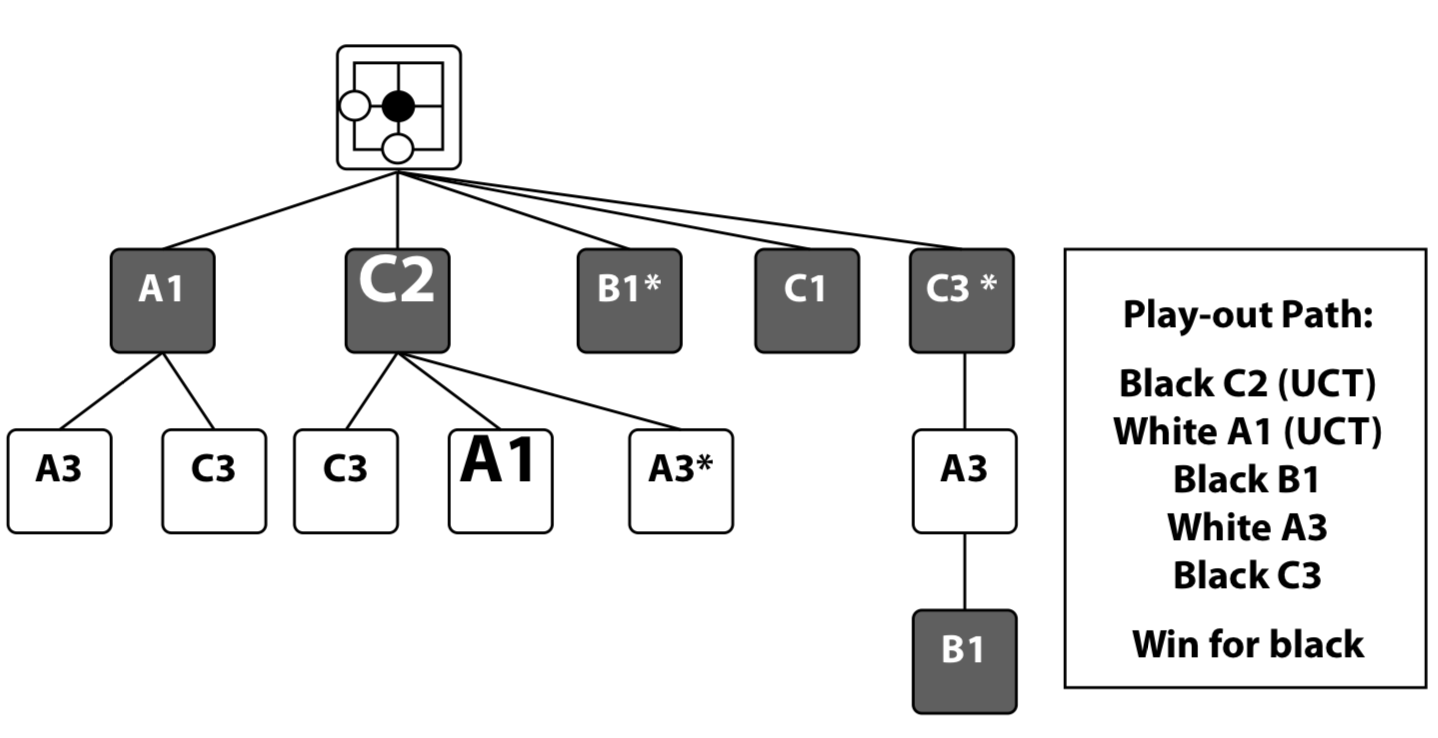
\includegraphics[width=\textwidth]{pictures/AMAF.png}
\end{center}
\caption[AMAF heuristic]{AMAF heuristic \cite{conf/icai/HelmboldP09}}
\label{fig:AMAFheuristic}
\end{figure}
In order to have both values, a separate count of rewards and visits for each type of update is maintained. So the total score of an action is expressed as

\begin{equation}
    \alpha A + (1 - \alpha) U
\end{equation}
where U represent the standard UCT score and A represent the AMAF score.
The value of $\alpha$ used at each node decrease with each visit and it is computed, supplying a fixed positive integer $V>0$, after \textit{n} visit as \cite{conf/icai/HelmboldP09}

\begin{equation}
    \max \left\{0,\frac{V - v(n)}{V}\right\}
\end{equation}
where parameter \textit{V} represent the maximum value of visits a node can have in order to use the RAVE values to correct the UCT score; when a node is visited more times than the value expressed by \textit{V}, RAVE values are not being used at all. With this approach exploited areas of the tree will use the accurate statistics more that unexplored areas of the tree.

\subsection{Node Elimination}
In addition to known enhancements we propose a new method to improve MCTS performance in domains with many early terminal states. One such domain is Sokoban, in which earlier deadlock detection can significantly reduce the search space. The idea behind \textit{Node Elimination} is based on the observation that MCTS often repeatedly selected nodes that would lead to a deadlock inside the tree. This was caused by the constraints posed by the problem itself and we will therefore use Sokoban to illustrate the concept of Node Elimination.

\medskip\noindent
In a Sokoban search, every rollout can end in either a solved state or a deadlock. With deadlocks being far more likely in non trivial levels, penalizing the reward of every rollout that terminated in a deadlock would not be beneficial to the search, since the hard part is not minimizing the cost to the solution but actually finding the solution. Furthermore, the length of the rollout does not give any insight on the quality of the rollout, since the move that originally caused a deadlock might have been executed far before the deadlock was finally detected. This lead to nodes close to the root being selected many times despite representing a deadlock state, wasting search resources. The solution we propose to this kind of situation is a recursive Node Elimination starting from terminal states.

\medskip\noindent
During the backpropagation phase we remove from the tree all nodes in the current path that have no children and no untried moves. Terminal nodes are therefore directly eliminated (as they never have untried moves), effectively removing all deadlocks from the tree. When a node is eliminated it's also removed from its parent's list of children, therefore if every child of a node is a deadlock, that node is removed too. This goes on recursively, removing dead sub-trees that have already been fully explored. The elimination process is illustrated in figure \ref{fig:nodeelimination}.
\begin{figure}[ht]
    \centering
    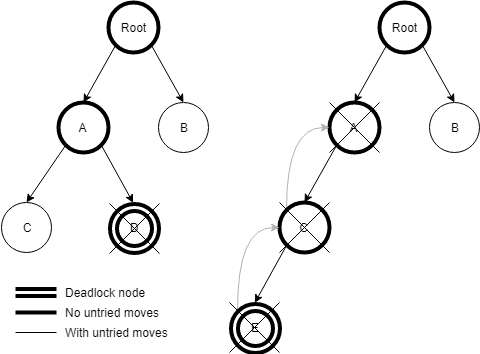
\includegraphics[width=0.9\linewidth]{pictures/NodeElimination.png}
        \caption[Node elimination]{Node elimination:\\
            Simple Node Elimination (left): only node D can be removed because node A still has children.
             Recursive Node Elimination (right): node C is expanded into terminal node E and --- after the 0-length rollout --- nodes E, C and A can be removed because once one is removed, its parent is left with no children and no untried moves.}
    \label{fig:nodeelimination}
\end{figure}
Node Elimination was also combined with Node Recycling by removing eliminated nodes from the node pool.

\medskip\noindent
While in most two-player games, revisiting the same terminal nodes can be beneficial to the accuracy of the evaluation of the best move, in single player games the only required information is the top score achieved among all rollouts. Therefore, once a path has been fully explored it's no longer needed and can be ignored for the rest of the search. In the context of puzzle games, Node Elimination should provide the largest improvements in domains where terminal states can appear early in the search.

\subsection{Cycles Avoidance}
When working in domains where the game tree contains many cycles it's important to keep track of the visited states in the current path to ensure that no state is visited more than once, otherwise the search can enter loops and waste computational resources. In our SP-MCTS implementation we keep track of all visited states in the iteration, from the root to the end of the simulation. When selecting a move for expanding a node or for performing the rollout, we check if the resulting state has already been visited in the current path. If it is, we considered two options:
\begin{itemize}
    \item \textit{Stop On Cycle}: whether the cycle is encountered during the expansion phase or the simulation phase, the search treats the last state as terminal and immediately performs the packpropagation phase.
    \item \textit{Avoid Cycles}: the algorithm tries different moves among those available in the current state until either a valid non-visited state is obtained, or no more moves are available. If a valid state is obtained, the corresponding move is selected, otherwise the iteration is stopped.
\end{itemize}

\section{Sokoban optimizations}
In order to test the performance of the algorithm on Sokoban we had to implement some domain specific optimizations to reduce the search tree. These are some of the optimizations that were briefly described in Section \ref{sokobanoptimizations}.

\subsection{Push Level Search}
In Sokoban the pusher can move freely on the board but in reality the only relevant moves are those that change the position of a box. This means that instead of performing the search on states resulting from a single move, we perform it on an abstract layer in which each high-level move is actually a sequence of basic moves that ends with a box being pushed. In order to generate these high level moves, we need to perform local searches to identify the squares that the player can reach and from which he can push a box. These local searches are performed as breadth first searches on the low-level representation of the state. This solution can increase the branching factor if the player can reach many boxes from different directions, but it greatly reduces depth and minimizes the occurrence of cycles, reducing the overhead introduced by cycle avoidance.

\subsection{Deadlock Detection}
In addition to the abstract representation of the board, the first and fundamental optimization required is deadlock detection. We employed two different techniques to identify two types of deadlock: simple deadlocks and freeze deadlocks.

\medskip\noindent
Simple deadlocks consist in a set of squares from which a stone can't reach any goal. They are computed only once, upon creation of the state object. To find them, a series of breadth first searches are performed: starting from each goal, the pusher is moved as if it was pulling a box instead of pushing it. It tries to pull in every direction into adjacent squares and recursively repeats the process for every new square encountered. During the search, all squares from which the pusher can pull a box are marked as visited, and represent all positions from which the box can reach that goal. After the search has been executed for each goal, the squares that are not marked as visited are those from which no box can reach a goal and will be kept in a hash table for the duration of the search. Whenever a box is pushed to one of those squares the state is flagged as a deadlock.

\medskip\noindent
Freeze deadlock are identified during the search since they depend on the configuration of multiple boxes. A box is considered frozen if it can't move neither horizontally nor vertically. A box can't move horizontally if it has a wall on either side, or a frozen box. When a box is pushed to be adjacent to another box, we check if the box we just pushed is frozen, and in order to establish that we need to check if adjacent boxes are frozen. If any one of the chain of boxes is frozen, the state is a deadlock.

\subsection{Tunnel Macros}
Tunnel Macros are used to merge multiple pushes into a single move. They reduce tree depth and can help avoid deadlocks that would occur by pushing two boxes into the same tunnel.
A tunnel can be defined as a portion of the level in which a line of squares is surrounded by walls. Every time available moves are generated, if the pattern of box and walls matches the one shown in Figure \ref{fig:tunnelmacro}, instead of a single push, a series of pushes is generated, equal to the number of squares required to place the box out of the tunnel. The only exception to this rule is if the tunnel contains a goal; in this case the box can be stopped on the goal (shown in figure \ref{fig:tunnelmacroexception}).
\begin{figure}[ht]
    \centering
    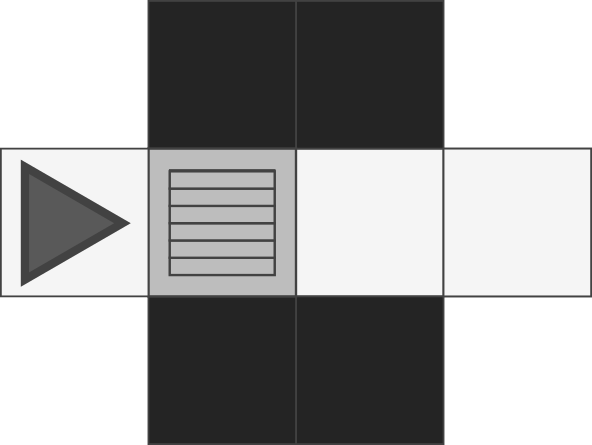
\includegraphics[width=0.4\linewidth]{pictures/TunnelMacro.png}
    \caption[Tunnel Macro]{Tunnel Macro\\ Instead of R, the move RR is generated}
    \label{fig:tunnelmacro}
\end{figure}
\begin{figure}[ht]
    \centering
    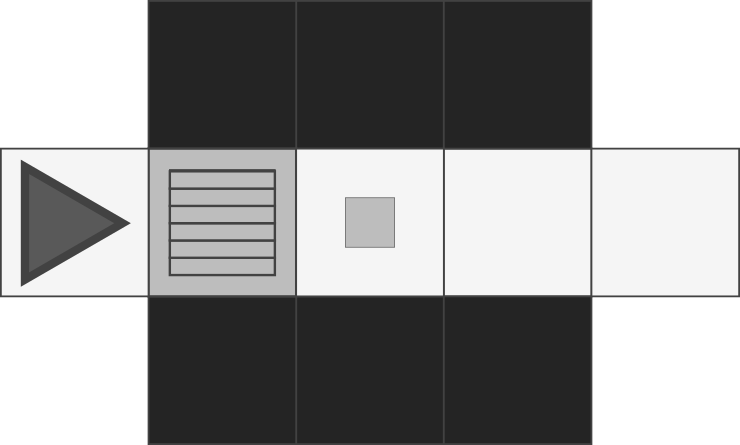
\includegraphics[width=0.5\linewidth]{pictures/TunnelMacroException.png}
    \caption[Tunnel Macro Exception]{Tunnel Macro Exception\\ The move R is generated to push the box on the goal. The next time available moves are computed, move RR will be generated}
    \label{fig:tunnelmacroexception}
\end{figure}

\subsection{Goal Macros}
Goal Macros are used to identify the order with which goals are covered by boxes inside a goal room. A goal room is an area of the board with at least three adjacent boxes, which tries to maximize the number of squares and minimize the number of entrances and the number of boxes, according to the following formula
\begin{equation}
    GRoomScore = 1000*(20-en)+5*sq- 100*man\_io- 500*boxes
\end{equation}
where $en$ is the number of entrances, $sq$ is the number of squares, $man\_io$ are entrances from which the pusher can enter the goal room but he cannot push a box through and $boxes$ is the number of boxes inside the goal room. If a suitable goal room is found, the next step is to build the Goal Macro Tree. The Goal Macro Tree contains for each node a hash that represents the boxes on the goal room's goals, a sequence of pairs entrance-goal that represent the goal that the box should be pushed to if it was on that entrance and a sequence of moves that can be used to execute the macro. During moves generation, if a box is about to be pushed to an entrance square, the tree is accessed to retrieve the move sequence. If the move sequence is valid in the current state, it's substituted to the single push. If the sequence is not valid, an online search is executed by considering a sub-problem in which every other box is turned into a wall and the only valid goal is the one that should be filled by the macro. If the search is successful, the sequence is used as a macro, otherwise the single push is used.

\subsection{Goal Cuts}
Goal Cuts are a simple improvement over Goal Macros for which instead of adding the Goal Macro to the list of available moves in the current states, it is returned as the only move available.